\section{What is Software-Defined Networking?}

The term SDN (Software-Defined Networking)  was originally coined to represent 
the ideas and work around OpenFlow at Stanford University~\cite{greene2009}. 
As originally defined, SDN refers to a network architecture where the forwarding 
state in the data plane is managed by a remote control plane decoupled from the former.
The networking industry has on many occasions shifted from this original view of SDN, 
by referring to anything that involves software as being SDN. We therefore attempt, 
in this section, to provide a much less ambiguous definition of software-defined 
networking.

%SDN: key characteristics.
We define an SDN as a network archi\-te\-cture with four pillars:\\
\begin{enumerate}
\item  The control and data planes are \textit{decoupled}. Control functionality is 
removed from network devices that will become simple (packet) forwarding elements.
\item  Forwarding decisions are flow-based, instead of des\-ti\-na\-tion-based. A flow is 
broadly defined by a set of packet field values acting as a match (filter) criterion 
and a set of actions (instructions). The flow abstraction allows unifying the behavior of 
different types of network devices, including routers, switches, firewalls, and middleboxes. 
Flow programming enables unprecedented flexibility, limited only to the capabilities of 
the implemented flow tables~\cite{mckeown2008}.
\item Control logic is moved to an external entity, the so-called SDN controller or Network 
Operating System (NOS). The NOS is a software platform that runs on commodity server technology 
and provides the essential resources and abstractions to facilitate the programming of forwarding 
devices based on a logically centralized, abstract network view. Its purpose is therefore similar 
to that of a traditional operating system.
\item The network is \textit{programmable} through software applications running on top of the NOS that 
interacts with the underlying data plane devices. This is a fundamental characteristic of SDN, considered 
as its main value proposition.
\end{enumerate}

Note that the logical centralization of the control logic, in particular, offers several 
additional benefits.  First, it is simpler and less error-prone to modify network policies 
through high-level languages and software components, compared with low-level device specific
configurations. Second, a control program can automatically react to spurious changes of the 
network state and thus maintain the high-level policies intact. Third, the centralization of 
the control logic in a controller with global knowledge of the network state simplifies the
development of more sophisticated networking functions, services and applications.

Following the SDN concept~\cite{schenker2011}, an SDN can be defined by 
three fundamental abstractions: (\textit{i}) forwarding, (\textit{ii}) distribution, and 
(\textit{iii}) specification.
In fact, abstractions are essential tools of research in computer science and information technology, being already an ubiquitous feature of many computer architectures and systems~\cite{alkhatib2014}.


Ideally, the \textit{forwarding abstraction} should allow any forwarding behavior desired 
by the network application (the control program) while hiding details of the underlying hardware.
OpenFlow is a practical realization of one such abstraction, which can be seen as the equivalent 
to a ``device driver'' in an operating system.

The \textit{distribution abstraction} should shield SDN applications from the vagaries 
of distributed state, making the distributed control problem a logically centralized one.  Its
realization requires a common distribution layer, which in SDN resides in the NOS. This layer has 
two essential functions. First, it is responsible for installing the control commands on the 
forwarding devices.  Second, it collects status information about the forwarding layer (network 
devices and links), to offer a global network view to network applications.

The last abstraction is \textit{specification}, which should allow a network application to express 
the desired network behavior without being responsible for implementing that behavior itself.
This can be achieved through virtualization solutions, as well as network programming languages.
These approaches map the abstract configurations that the applications express based on a simplified, 
abstract model of the network, into a physical configuration for the global network view exposed by 
the SDN controller. Figure~\ref{fig:sdn_abstractions} depicts the SDN architecture, concepts and 
building blocks.
%illustrates these ideas pictorially.
% Note: maybe, it could be a good idea to give a more practical example for "specification abstractions". Maybe something related with the last paper of Jen (USENIX Login). Example: an abstraction could be a view of the network as a single big switch, mapped on a set of physical devices (e.g. four switches).

\begin{figure}[t!]
\centering
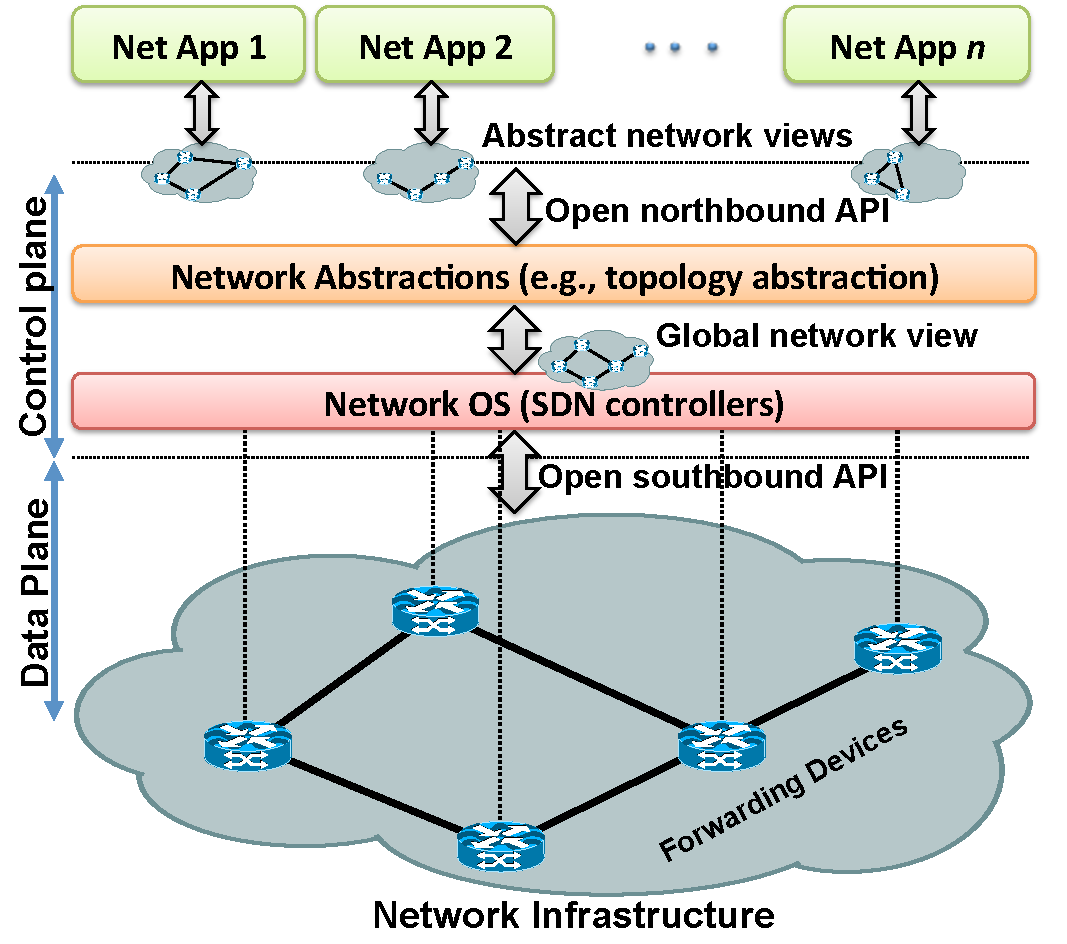
\includegraphics[width=0.95\columnwidth]{figures/fig3_sdn_abstractions.pdf}
\caption{SDN architecture and its fundamental abstractions.}
\label{fig:sdn_abstractions}
\end{figure}

As previously mentioned, the strong coupling between control and data planes has made it difficult 
to add new functionality to traditional networks. The introduction of new features requires the 
inclusion of expensive and hard-to-configure equipment in the network -- load balancers, intrusion detection systems and firewalls 
are common examples. These middleboxes need to be placed strategically in the network, making it 
even harder to later change the network topology, configuration and functionality. 
This can be observed in Figure~\ref{fig:traditionalversusSDN}.
For instance, an intrusion detection system might need to receive a cloned copy of the traffic of all switching devices of the network through specific physical and or logical links.
%Moreover, these specialized devices have usually to be configured in a standalone or specific way because each of them has its own (most of time proprietary) interface and configuration protocols.
%On the former we have a strong coupling between control and data planes.
%Appliances such as firewalls and load balancers have to be installed in specific physical spots of the network.
%Moreover, forwarding devices are managed separately from other elements of the network, adding diversity and complexity to the network management and operation tasks.

\begin{figure}[t!]
\centering
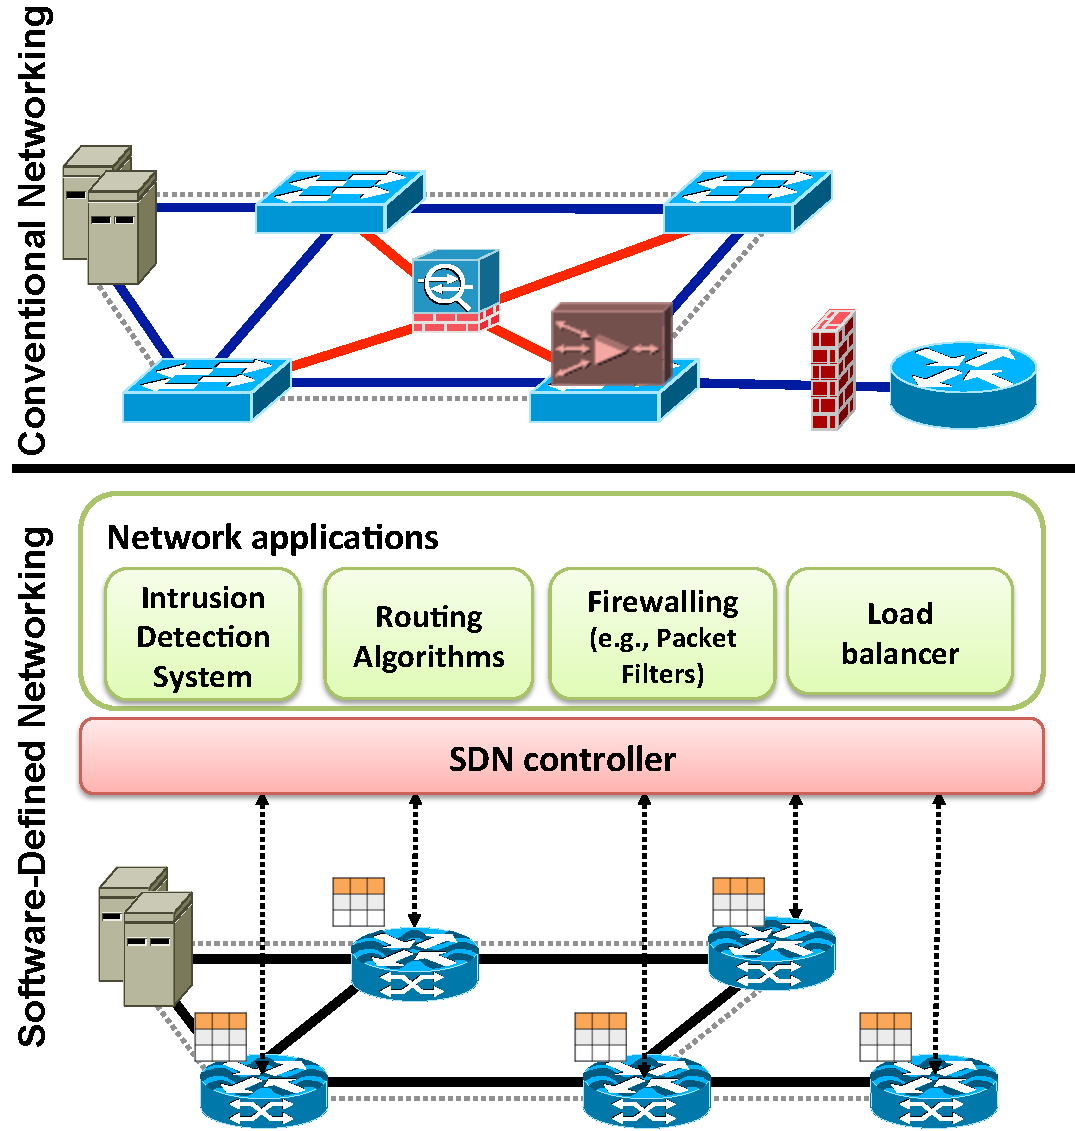
\includegraphics[width=0.95\columnwidth]{figures/fig4_traditional_and_sdn.pdf}
\caption{Traditional networks versus Software-Defined Networks (SDNs). With SDN, management becomes simpler and traditional middleboxes can be removed.}
\label{fig:traditionalversusSDN}
\end{figure}

In contrast, introducing new functionality in SDN is made simply by adding a new software 
application to run on top of the NOS. This approach has several advantages:
\begin{itemize}
\item It becomes easier to program these applications since the abstractions provided by the 
control platform and/or the network programming languages can be shared.
\item All applications can take advantage of the same network information (the global network view), 
leading (arguably) to more consistent and effective policy decisions while re-using control plane 
software modules.
\item These applications can take actions (i.e., reconfigure forwarding devices) from any part of 
the network. There is therefore no need to devise a precise strategy about the location of the new 
functionality.
\item The integration of different applications becomes more straightforward. For instance, load 
balancing and routing applications can be combined sequentially, with load balancing decisions having 
precedence over routing policies.
\end{itemize}
%Essentially, an SDN data plane is comprised of forwarding devices devoid of intelligence.
%Their only task is to process incoming packets based on match and action rules defined by applications running on top of controllers.
%A logically-centralized controller, or network operating system (NOS), abstracts the network for the applications, providing a global view that makes the network look like a single big switch or router.
%The NOS is responsible of dealing with the data collection and distribution to and from data plane devices.
%This data is basically of three types: (1) configuration and forwarding rules sent by the controller to program the device; (2) requests from data plane devices; (3) statistics from the network requested/sent through push or pull interfaces.
%
%In the SDN world OpenFlow is an open standard developed to materialize the clear separation between control and data plane functionalities.
%A controller keeps communication channels with data plane devices, through which it sends and receives OpenFlow messages.
%Forwarding devices can send the first packet of a flow to the controller when they do not know what to do with it.
%These requests are passed up to applications that implement the control logic.
%Their task is to analyze the request, look for policies to be applied and generate rules to be installed on the forwarding elements of the network.

%A data plane device's request can trigger the installation of flow rules in multiple devices.
%For instance, packets of a new flow A should routed to a service B.
%To setup the flow path the controller will have to program all forwarding devices up to service B.
%The forwarding rules are installed in a flow table, used by the device for matching incoming packets and take respective actions (e.g. forward, drop).
%Thereupon, the controller can be seen as  a general purpose network policy enforcement point.
%
%
%Finally, SDN is not a new concept.
%The first initiatives to separate control and data plane date back to the 80s, such as the AT\&T's network control point (NCP)~\cite{sheinbein1982}.
%Similarly, the first programmable data plane devices were introduced still in the 90s (e.g., active networks~\cite{tennenhouse1997}).
%
%\note{CH: May be include a discussion on what is NOT SDN. Introduce the SDN taxonomy by Srini here and/or defer the discussion to the Section on History of SDN?}
%\note{DK: Yes, that could be interesting. I think it fits better in the history section.}

\subsection{Terminology}

To identify the different elements of an SDN as unequivocally as possible, we now present the 
essential terminology used throughout this work.

\noindent \textit{Fowarding Devices (FD)}: Hardware- or software-based data plane devices that perform 
a set of elementary operations. The forwarding devices have well-defined instruction sets (e.g., flow 
rules) used to take actions on the incoming packets (e.g., forward to specific ports, drop, forward to 
the controller, rewrite some header). These instructions are defined by southbound interfaces (e.g., 
OpenFlow~\cite{mckeown2008}, ForCES~\cite{doria2010}, Protocol- Oblivious Forwarding (POF)~\cite{song2013}) and are installed in the forwarding devices by the SDN controllers implementing the southbound protocols.

\noindent \textit{Data Plane (DP)}: Forwarding devices are interconnected through wireless radio channels 
or wired cables. The network infrastructure comprises the interconnected forwarding devices, which 
represent the data plane.
%More specifically, the data plane is the part of the forwarding device which is responsible for receiving and sending packets across the data plane.

\noindent \textit{Southbound Interface (SI)}: The instruction set of the forwarding devices is defined 
by the southbound API, which is part of the southbound interface. Furthermore, the SI also defines the 
communication protocol between forwarding devices and control plane elements. This protocol formalizes 
the way the control and data plane elements interact.

\noindent \textit{Control Plane (CP)}: Forwarding devices are programmed by control plane elements 
through well-defined SI embodiments. The control plane can therefore be seen as the ``network brain''.
All control logic rests in the applications and controllers, which form the control plane.
%At the lowest layer of the control plane, there are southbound interfaces for sending and receiving requests from and to forwarding devices.
%These requests can contain flow control rules to be installed on forwarding devices, or action requests and statistics sent by forwarding devices to control plane elements, such as network operating systems.

\noindent \textit{Northbound Interface (NI)}: The network operating system can offer an API to application 
developers. This API represents a northbound interface, i.e., a common interface for developing applications.
%and interacting with external system such as cloud orchestration services.
Typically, a northbound interface abstracts the low level instruction sets used by southbound interfaces 
to program forwarding devices.

\noindent \textit{Management Plane (MP)}: The management plane is the set of applications that leverage 
the functions offered by the NI to implement network control and operation logic.
This includes applications such as routing, firewalls, load balancers, monitoring, and so on.
%In other words, the MP accommodates management applications which are responsible for programming, configuring and monitoring the network operation.
Essentially, a management application defines the policies, which are ultimately translated to 
southbound-specific instructions that program the behavior of the forwarding devices.

\subsection{Alternative/Broadening SDN Definitions}
\label{sec:alt-SDN}


Since its inception in 2010~\cite{greene2009}, the original OpenFlow-centered SDN term 
has seen its scope broadened beyond architectures with a cleanly decoupled control plane 
interface. The definition of SDN will likely continue to broaden, driven by the industry 
business-oriented views on SDN -- irrespective of the decoupling of the control plane. In 
this survey, we focus on the original, ``canonical'' SDN definition based on the aforementioned
key pillars and the concept of layered abstractions. However, for the sake of completeness 
and clarity, we acknowledge alternative SDN definitions~\cite{nadeau2013}, including:

%\begin{itemize}
%\item
\noindent \textit{Control Plane / Broker SDN}: A networking approach that retains existing distributed 
control planes but offers new APIs that allow applications to interact (bidirectionally) with the network. 
An SDN controller -- often called orchestration platform -- acts as a broker between the applications and 
the network elements. This approach effectively presents control plane data to the application and allows 
a certain degree of network programmability by means of ``plug-ins'' between the orchestrator function and 
network protocols. This API-driven approach corresponds to a hybrid model of SDN, since it enables the broker 
to manipulate and directly interact with the control planes of devices such as routers and switches. Examples 
of this view on SDN include recent IETF efforts (e.g., ALTO~\cite{alimi2013}, I2RS~\cite{ietfi2rsworkinggroup2014}, ABNO~\cite{king2014}) and the design philosophy behind the OpenDaylight project~\cite{opendaylight2013} that goes beyond the OpenFlow split control mode.

%\item 
\noindent \textit{Overlay SDN}: A networking approach where the (software- or hardware-based) network edge 
is dynamically programmed to manage tunnels between hypervisors and/or network switches, introducing an 
overlay network. In this hybrid networking approach, the distributed control plane providing the underlay 
remains untouched. The centralized control plane provides a logical overlay that utilizes the underlay 
as a transport network. This flavor of SDN follows a proactive model to install the overlay tunnels. The overlay
tunnels usually terminate inside virtual switches within hypervisors or in physical devices acting as gateways 
to the existing network. This approach is very popular in recent data center network virtualization \cite{chowdhury2010}, and are based on a variety of tunneling technologies (e.g., STT, NVGRE, VXLAN,
LISP)~\cite{jain2013}.

%\end{itemize}

In addition, the term SDN is often used to define extensible network management planes (e.g., OpenStack~\cite{corradi2014}), 
whitebox switches and open-source dataplanes (e.g., Pica8 Xorplus~\cite{shang2014}, Quagga~\cite{jakma2014}), specialized programmable hardware devices (e.g., 
NetFPGA~\cite{netfpga2014}), virtualized software-based appliances (e.g., Network Function Virtualization - NFV~\cite{martins2014}), in spite of 
lacking a decoupled control and data plane or common interface along its API. Hybrid SDN models will be further discussed in Section~\ref{sec:hybrid}. 
